\documentclass[aspectratio=169,10pt]{beamer}
\usepackage{fontspec}
\setsansfont{texgyreheros}[Extension=.otf,UprightFont=*-regular,BoldFont=*-bold,ItalicFont=*-italic,BoldItalicFont=*-bolditalic]
\setmainfont{texgyreheros}[Extension=.otf,UprightFont=*-regular,BoldFont=*-bold,ItalicFont=*-italic,BoldItalicFont=*-bolditalic]
\usepackage{booktabs,amsmath,tikz,tabularx}
\usetikzlibrary{arrows.meta,positioning,calc}
\graphicspath{{../results/figures/}}
\newcommand{\DiceClassicalFull}{0{,}561}
\newcommand{\JacClassicalFull}{0{,}420}
\newcommand{\HdClassicalFull}{40{,}69}
\newcommand{\AsdClassicalFull}{9{,}31}
\newcommand{\VolClassicalFull}{54{,}4}
\newcommand{\DiceUnetFull}{0{,}912}
\newcommand{\JacUnetFull}{0{,}838}
\newcommand{\HdUnetFull}{8{,}22}
\newcommand{\AsdUnetFull}{1{,}71}
\newcommand{\VolUnetFull}{6{,}5}
\newcommand{\DiceSdUnetFull}{0{,}001}
\newcommand{\DiceUnetFew}{0{,}828}
\newcommand{\JacUnetFew}{0{,}716}
\newcommand{\HdUnetFew}{19{,}55}
\newcommand{\AsdUnetFew}{3{,}57}
\newcommand{\VolUnetFew}{17{,}3}
\newcommand{\DiceSdUnetFew}{0{,}013}
\newcommand{\DiceDinoFull}{0{,}902}
\newcommand{\JacDinoFull}{0{,}822}
\newcommand{\HdDinoFull}{11{,}02}
\newcommand{\AsdDinoFull}{1{,}90}
\newcommand{\VolDinoFull}{5{,}9}
\newcommand{\DiceSdDinoFull}{0{,}002}
\newcommand{\DiceDinoFew}{0{,}849}
\newcommand{\JacDinoFew}{0{,}740}
\newcommand{\HdDinoFew}{20{,}55}
\newcommand{\AsdDinoFew}{3{,}50}
\newcommand{\VolDinoFew}{14{,}4}
\newcommand{\DiceSdDinoFew}{0{,}003}
\newcommand{\DiceMriFull}{0{,}908}
\newcommand{\JacMriFull}{0{,}832}
\newcommand{\HdMriFull}{7{,}82}
\newcommand{\AsdMriFull}{1{,}66}
\newcommand{\VolMriFull}{7{,}2}
\newcommand{\DiceSdMriFull}{0{,}001}
\newcommand{\DiceMriFew}{0{,}849}
\newcommand{\JacMriFew}{0{,}744}
\newcommand{\HdMriFew}{13{,}85}
\newcommand{\AsdMriFew}{2{,}80}
\newcommand{\VolMriFew}{11{,}7}
\newcommand{\DiceSdMriFew}{0{,}002}
\newcommand{\DiceConcatFull}{0{,}912}
\newcommand{\JacConcatFull}{0{,}839}
\newcommand{\HdConcatFull}{8{,}13}
\newcommand{\AsdConcatFull}{1{,}64}
\newcommand{\VolConcatFull}{6{,}1}
\newcommand{\DiceSdConcatFull}{0{,}001}
\newcommand{\DiceConcatFew}{0{,}864}
\newcommand{\JacConcatFew}{0{,}762}
\newcommand{\HdConcatFew}{14{,}75}
\newcommand{\AsdConcatFew}{2{,}86}
\newcommand{\VolConcatFew}{9{,}7}
\newcommand{\DiceSdConcatFew}{0{,}003}
\newcommand{\DiceGateFull}{0{,}911}
\newcommand{\JacGateFull}{0{,}838}
\newcommand{\HdGateFull}{7{,}43}
\newcommand{\AsdGateFull}{1{,}60}
\newcommand{\VolGateFull}{6{,}2}
\newcommand{\DiceSdGateFull}{0{,}002}
\newcommand{\DiceGateFew}{0{,}857}
\newcommand{\JacGateFew}{0{,}753}
\newcommand{\HdGateFew}{14{,}67}
\newcommand{\AsdGateFew}{2{,}86}
\newcommand{\VolGateFew}{12{,}4}
\newcommand{\DiceSdGateFew}{0{,}004}
\newcommand{\DiceGateEdgeFull}{0{,}913}
\newcommand{\JacGateEdgeFull}{0{,}840}
\newcommand{\HdGateEdgeFull}{7{,}52}
\newcommand{\AsdGateEdgeFull}{1{,}57}
\newcommand{\VolGateEdgeFull}{6{,}6}
\newcommand{\DiceSdGateEdgeFull}{0{,}001}
\newcommand{\DiceGateEdgeFew}{0{,}862}
\newcommand{\JacGateEdgeFew}{0{,}761}
\newcommand{\HdGateEdgeFew}{14{,}23}
\newcommand{\AsdGateEdgeFew}{2{,}80}
\newcommand{\VolGateEdgeFew}{10{,}6}
\newcommand{\DiceSdGateEdgeFew}{0{,}009}
\newcommand{\DicePpUnetFull}{0{,}914}
\newcommand{\HdPpUnetFull}{6{,}32}
\newcommand{\VolPpUnetFull}{6{,}7}
\newcommand{\DicePpUnetFew}{0{,}841}
\newcommand{\HdPpUnetFew}{12{,}50}
\newcommand{\VolPpUnetFew}{15{,}7}
\newcommand{\DicePpDinoFull}{0{,}908}
\newcommand{\HdPpDinoFull}{7{,}10}
\newcommand{\VolPpDinoFull}{6{,}4}
\newcommand{\DicePpDinoFew}{0{,}861}
\newcommand{\HdPpDinoFew}{14{,}70}
\newcommand{\VolPpDinoFew}{14{,}4}
\newcommand{\DicePpMriFull}{0{,}910}
\newcommand{\HdPpMriFull}{6{,}47}
\newcommand{\VolPpMriFull}{7{,}4}
\newcommand{\DicePpMriFew}{0{,}859}
\newcommand{\HdPpMriFew}{9{,}71}
\newcommand{\VolPpMriFew}{11{,}1}
\newcommand{\DicePpConcatFull}{0{,}915}
\newcommand{\HdPpConcatFull}{6{,}76}
\newcommand{\VolPpConcatFull}{6{,}5}
\newcommand{\DicePpConcatFew}{0{,}876}
\newcommand{\HdPpConcatFew}{9{,}72}
\newcommand{\VolPpConcatFew}{8{,}8}
\newcommand{\DicePpGateFull}{0{,}914}
\newcommand{\HdPpGateFull}{5{,}82}
\newcommand{\VolPpGateFull}{6{,}4}
\newcommand{\DicePpGateFew}{0{,}868}
\newcommand{\HdPpGateFew}{10{,}82}
\newcommand{\VolPpGateFew}{11{,}4}
\newcommand{\DicePpGateEdgeFull}{0{,}915}
\newcommand{\HdPpGateEdgeFull}{6{,}15}
\newcommand{\VolPpGateEdgeFull}{7{,}1}
\newcommand{\DicePpGateEdgeFew}{0{,}872}
\newcommand{\HdPpGateEdgeFew}{10{,}51}
\newcommand{\VolPpGateEdgeFew}{10{,}1}
\newcommand{\PGateVsDinoFull}{{=}0{,}001}
\newcommand{\WinGateVsDinoFull}{18/20}
\newcommand{\DiffGateVsDinoFull}{+0{,}009}
\newcommand{\PGateVsMriFull}{{=}0{,}001}
\newcommand{\WinGateVsMriFull}{16/20}
\newcommand{\DiffGateVsMriFull}{+0{,}003}
\newcommand{\PGateVsConcatFull}{{=}0{,}294}
\newcommand{\WinGateVsConcatFull}{8/20}
\newcommand{\DiffGateVsConcatFull}{-0{,}001}
\newcommand{\PConcatVsDinoFull}{{<}0{,}001}
\newcommand{\WinConcatVsDinoFull}{19/20}
\newcommand{\DiffConcatVsDinoFull}{+0{,}010}
\newcommand{\PMriVsDinoFull}{{=}0{,}036}
\newcommand{\WinMriVsDinoFull}{15/20}
\newcommand{\DiffMriVsDinoFull}{+0{,}006}
\newcommand{\PGateVsUnetFull}{{=}0{,}869}
\newcommand{\WinGateVsUnetFull}{10/20}
\newcommand{\DiffGateVsUnetFull}{-0{,}001}
\newcommand{\PDinoVsUnetFull}{{=}0{,}024}
\newcommand{\WinDinoVsUnetFull}{6/20}
\newcommand{\DiffDinoVsUnetFull}{-0{,}010}
\newcommand{\PMriVsUnetFull}{{=}0{,}231}
\newcommand{\WinMriVsUnetFull}{9/20}
\newcommand{\DiffMriVsUnetFull}{-0{,}004}
\newcommand{\PGateEdgeVsGateFull}{{=}0{,}097}
\newcommand{\WinGateEdgeVsGateFull}{13/20}
\newcommand{\DiffGateEdgeVsGateFull}{+0{,}002}
\newcommand{\PGateEdgeVsUnetFull}{{=}0{,}841}
\newcommand{\WinGateEdgeVsUnetFull}{11/20}
\newcommand{\DiffGateEdgeVsUnetFull}{+0{,}001}
\newcommand{\PGateVsDinoFew}{{=}0{,}154}
\newcommand{\WinGateVsDinoFew}{15/20}
\newcommand{\DiffGateVsDinoFew}{+0{,}008}
\newcommand{\PGateVsMriFew}{{=}0{,}956}
\newcommand{\WinGateVsMriFew}{10/20}
\newcommand{\DiffGateVsMriFew}{+0{,}008}
\newcommand{\PGateVsConcatFew}{{=}0{,}202}
\newcommand{\WinGateVsConcatFew}{8/20}
\newcommand{\DiffGateVsConcatFew}{-0{,}007}
\newcommand{\PConcatVsDinoFew}{{=}0{,}064}
\newcommand{\WinConcatVsDinoFew}{16/20}
\newcommand{\DiffConcatVsDinoFew}{+0{,}015}
\newcommand{\PMriVsDinoFew}{{=}0{,}165}
\newcommand{\WinMriVsDinoFew}{14/20}
\newcommand{\DiffMriVsDinoFew}{-0{,}000}
\newcommand{\PGateVsUnetFew}{{=}0{,}008}
\newcommand{\WinGateVsUnetFew}{16/20}
\newcommand{\DiffGateVsUnetFew}{+0{,}029}
\newcommand{\PDinoVsUnetFew}{{=}0{,}784}
\newcommand{\WinDinoVsUnetFew}{10/20}
\newcommand{\DiffDinoVsUnetFew}{+0{,}021}
\newcommand{\PMriVsUnetFew}{{=}0{,}030}
\newcommand{\WinMriVsUnetFew}{14/20}
\newcommand{\DiffMriVsUnetFew}{+0{,}021}
\newcommand{\PGateEdgeVsGateFew}{{=}0{,}133}
\newcommand{\WinGateEdgeVsGateFew}{13/20}
\newcommand{\DiffGateEdgeVsGateFew}{+0{,}006}
\newcommand{\PGateEdgeVsUnetFew}{{=}0{,}004}
\newcommand{\WinGateEdgeVsUnetFew}{16/20}
\newcommand{\DiffGateEdgeVsUnetFew}{+0{,}034}
\newcommand{\GateInside}{0{,}107}
\newcommand{\GateBoundary}{0{,}296}
\newcommand{\GateNear}{0{,}579}
\newcommand{\GateFar}{0{,}693}
\newcommand{\ClassicalSigma}{2}
\newcommand{\ClassicalK}{1{,}2}
\newcommand{\ClassicalR}{24}
\newcommand{\ParamsUnet}{1{,}94}
\newcommand{\ParamsDino}{0{,}20}
\newcommand{\ParamsGate}{0{,}30}
\newcommand{\ParamsGateEdge}{0{,}30}
\newcommand{\TrainMsDino}{50}
\newcommand{\TrainMsGate}{54}
\newcommand{\TrainMsGateEdge}{76}
\newcommand{\TrainMsUnet}{182}
\newcommand{\InferGate}{10{,}1}
\newcommand{\InferUnet}{0{,}3}
\newcommand{\ErrBand}{64}
\newcommand{\ErrEnds}{39}
\newcommand{\RefBand}{19}
\newcommand{\RefEnds}{19}
\newcommand{\GatePpRawDice}{0{,}911}
\newcommand{\GatePpRawHd}{7{,}43}
\newcommand{\GatePpLccDice}{0{,}912}
\newcommand{\GatePpLccHd}{6{,}24}
\newcommand{\GatePpLccFillDice}{0{,}912}
\newcommand{\GatePpLccFillHd}{6{,}19}
\newcommand{\GatePpLccFillCloseDice}{0{,}914}
\newcommand{\GatePpLccFillCloseHd}{5{,}82}


\definecolor{ptitred}{HTML}{C8102E}
\definecolor{ink}{HTML}{0B0B0B}
\definecolor{ink2}{HTML}{52514E}
\setbeamercolor{structure}{fg=ptitred}
\setbeamercolor{frametitle}{fg=ptitred,bg=white}
\setbeamercolor{normal text}{fg=ink}
\setbeamercolor{itemize item}{fg=ptitred}
\setbeamercolor{itemize subitem}{fg=ink2}
\setbeamerfont{frametitle}{series=\bfseries,size=\Large}
\setbeamertemplate{navigation symbols}{}
\setbeamertemplate{itemize items}[circle]
\setbeamertemplate{footline}{%
  \hbox to \paperwidth{\hspace{4mm}\color{ink2}\tiny GateFuse-LA \;|\; Xử lý ảnh -- PTIT\hfill\insertframenumber/\inserttotalframenumber\hspace{4mm}}\vspace{2mm}}
\setbeamertemplate{frametitle}{\vspace{2mm}\insertframetitle\par\vspace{-1mm}{\color{ptitred}\rule{\linewidth}{0.6pt}}}
\renewcommand{\figurename}{Hình}
\renewcommand{\tablename}{Bảng}

\newcommand{\hl}[1]{{\color{ptitred}\textbf{#1}}}

\begin{document}

%---------------------------------------------------------------- 1
\begin{frame}[plain]
\vspace{4mm}
{\small\color{ink2} HỌC VIỆN CÔNG NGHỆ BƯU CHÍNH VIỄN THÔNG -- KHOA TRÍ TUỆ NHÂN TẠO}\\[1mm]
{\small\color{ink2} Dự án môn Xử lý ảnh -- Lựa chọn 2: dự án xử lý ảnh thực tế}\\[10mm]
{\LARGE\bfseries\color{ptitred} GateFuse-LA}\\[3mm]
{\Large Hợp nhất có cổng đặc trưng tổng quát và đặc trưng chuyên MRI\\[1mm] cho phân đoạn tâm nhĩ trái trên ảnh LGE-MRI}\\[12mm]
{\small Giảng viên: PGS.TS. Phạm Văn Cường}\\[1mm]
{\small Lớp [XX] -- Nhóm [YY]: [Họ tên SV1], [SV2], [SV3], [SV4], [SV5]}\\[1mm]
{\small\color{ink2} Mã nguồn: github.com/scalliontor/image\_processing}
\end{frame}

%---------------------------------------------------------------- 2
\begin{frame}{Bài toán: tách khoang tâm nhĩ trái trên LGE-MRI}
\begin{columns}[T]
\column{0.48\textwidth}
\begin{itemize}
\item \textbf{Vào}: khối LGE-MRI $h\times w\times 88$ lát (voxel 0.625\,mm)
\item \textbf{Ra}: mặt nạ 3D của tâm nhĩ trái (LA)
\item \textbf{Dùng để}: đo thể tích nhĩ, dựng mô hình 3D, định vị sẹo trước khi đốt điện điều trị rung nhĩ; vẽ tay mất hàng giờ
\end{itemize}
\column{0.5\textwidth}
\hl{Khó khăn cốt lõi}
\begin{itemize}
\item Máu trong LA \emph{sáng ngang} tĩnh mạch phổi, động mạch chủ, buồng tim bên cạnh
\item Biên yếu, nhiễu; tương phản khác nhau giữa các ca
\item Nhánh tĩnh mạch phổi mảnh, hình dạng biến thiên
\item Nhãn từng voxel đắt $\Rightarrow$ cần học với \emph{ít nhãn}
\end{itemize}
\end{columns}
\vspace{2mm}
\centering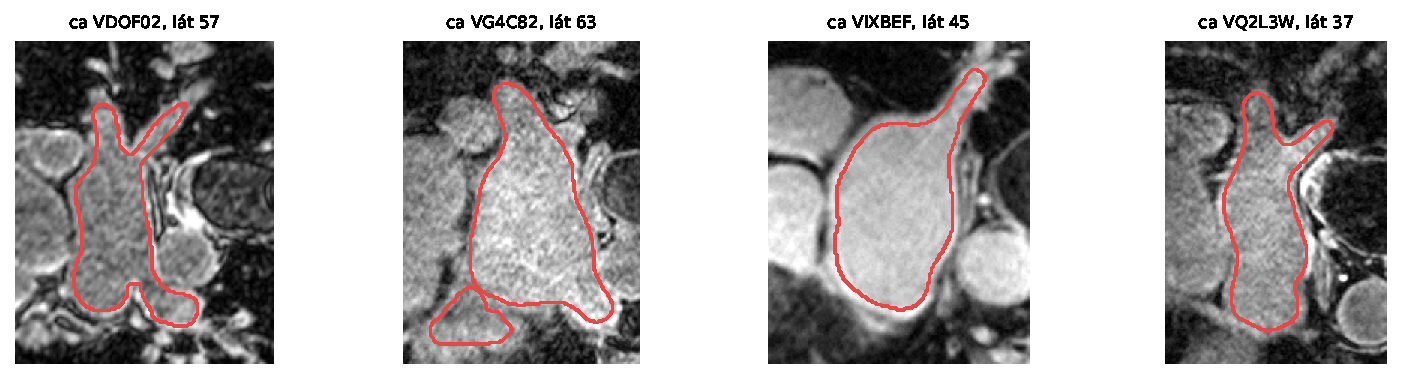
\includegraphics[width=0.86\linewidth]{data_examples.pdf}\\
{\scriptsize\color{ink2} Viền đỏ: nhãn chuyên gia trên 4 bệnh nhân của tập test -- tâm nhĩ dính liền các cấu trúc cùng độ sáng.}
\end{frame}

%---------------------------------------------------------------- 3
\begin{frame}{Ý tưởng: hai mô hình nền tảng, mỗi cái có một điểm mù}
\begin{columns}[T]
\column{0.56\textwidth}
\small
\renewcommand{\arraystretch}{1.3}
\begin{tabularx}{\linewidth}{@{}l>{\raggedright\arraybackslash}X>{\raggedright\arraybackslash}X@{}}
\toprule
 & \textbf{DINOv3 ViT-B/16} & \textbf{MRI-CORE ViT-B/16}\\
\midrule
Học từ & $\sim$1,7 tỷ ảnh tự nhiên & $\sim$6 triệu lát MRI\\
Mạnh ở & hình dạng, ngữ nghĩa & tương phản, nhiễu MRI\\
Điểm mù & chưa thấy MRI & dữ liệu không nhắc tới tim\\
\bottomrule
\end{tabularx}
\vspace{3mm}

\hl{GateFuse}: giữ \emph{đông cứng} cả hai encoder, học một \textbf{cổng theo từng điểm ảnh}\\[1mm]
\centerline{$g=\sigma\big(\mathrm{conv}[P_D,P_M]\big),\quad F=g\,P_D+(1-g)\,P_M$}\par\vspace{1mm}
\hl{D+}: GateFuse + nhánh biên Sobel ở độ phân giải đầy đủ (ch.\,5)
\column{0.42\textwidth}
\small
\hl{Câu hỏi nghiên cứu}
\begin{itemize}
\item[RQ1] Đặc trưng chuyên MRI có hơn đặc trưng tổng quát?
\item[RQ2] Ghép có bổ sung? Có cổng có hơn ghép nối?
\item[RQ3] Cổng tin encoder nào, ở vùng nào?
\item[RQ4] Chỉ có 8 khối có nhãn thì sao?
\item[RQ5] Xử lý ảnh cổ điển (ch.\,3, 5, 7) đóng góp bao nhiêu?
\end{itemize}
\end{columns}
\end{frame}

%---------------------------------------------------------------- 4
\begin{frame}{Dữ liệu và kiến thức học phần sử dụng}
\begin{columns}[T]
\column{0.5\textwidth}
\hl{2018 Atrial Segmentation Challenge} (bản .h5 của UA-MT)
\begin{itemize}
\item 100 khối LGE-MRI, nhãn tay của chuyên gia
\item Đã cắt quanh tâm nhĩ: $148\!\times\!132$ đến $244\!\times\!160$, 88 lát
\item Chia \textbf{theo ca bệnh}: 72 train / 8 validation / 20 test
\item Test: \textbf{1\,760 lát} (1\,231 lát có tâm nhĩ) $\gg$ 50 ảnh
\item Chế độ ít nhãn: chỉ \textbf{8 khối} (10\%)
\end{itemize}
\column{0.5\textwidth}
\small
\begin{tabularx}{\linewidth}{Xc}
\toprule
Kỹ thuật & Chương\\
\midrule
Cắt phân vị, kéo giãn min--max, đệm, nội suy & 2, 3\\
Lọc Gauss 3D & 3\\
Phân ngưỡng Otsu & 5\\
Phép mở/đóng, TPLT, lấp lỗ & 7\\
PCA đặc trưng & 8\\
Dice, HD95 qua biến đổi khoảng cách & 5, 7\\
\bottomrule
\end{tabularx}
\end{columns}
\end{frame}

%---------------------------------------------------------------- 5
\begin{frame}{Pipeline GateFuse-LA}
\centering
\resizebox{\linewidth}{!}{% Pipeline diagram shared by the report and the slides (needs tikz + arrows.meta, positioning)
\begin{tikzpicture}[
  font=\sffamily\scriptsize, >=Stealth, node distance=3mm and 4mm,
  box/.style={draw=black!55, rounded corners=2pt, align=center, inner sep=3pt, minimum height=9mm, fill=white},
  stage/.style={box, fill=ptitred!8},
  enc/.style={box, minimum width=27mm},
  arr/.style={->, thick, black!65},
  lab/.style={font=\sffamily\tiny, text=black!60}]
  \node[stage] (in) {Khối LGE-MRI\\$h\times w\times 88$};
  \node[stage, right=of in] (pre) {Tiền xử lý (ch.\,2--3)\\cắt percentile 0.5--99.5\\min--max theo lát\\đệm 256, phóng $\times2$};
  \node[enc, right=6mm of pre, yshift=7mm, fill=blue!7] (dino) {DINOv3 ViT-B/16\\(đông cứng, ảnh tự nhiên)};
  \node[enc, right=6mm of pre, yshift=-7mm, fill=orange!10] (mri) {MRI-CORE ViT-B/16\\(đông cứng, 6\,tr lát MRI)};
  \node[box, right=13mm of dino] (pd) {chiếu $1{\times}1$\\$P_D$};
  \node[box, right=13mm of mri] (pm) {chiếu $1{\times}1$\\$P_M$};
  \path (pd.east) -- (pm.east) coordinate[midway] (mid);
  \node[box, right=6mm of mid, fill=green!8] (gate) {Cổng học được\\$g=\sigma(\mathrm{conv}[P_D,P_M])$\\$F=g P_D+(1-g)P_M$};
  \node[box, right=of gate] (dec) {Decoder\\$32\to256$};
  \node[stage, right=of dec] (post) {Hậu xử lý (ch.\,7)\\ngưỡng 0.5\\TPLT 3D lớn nhất\\lấp lỗ};
  \node[box, below=4mm of post] (out) {Mặt nạ 3D\\Dice, Jaccard\\HD95, ASD};
  \node[box, dashed, fill=violet!6, below=9mm of gate] (det) {Nhánh chi tiết (D+)\\ảnh + gradient Sobel (ch.\,5)\\2 lớp conv ở $256{\times}256$};
  \draw[arr] (in) -- (pre);
  \draw[arr] (pre.east) -- ++(3mm,0) |- (dino.west);
  \draw[arr] (pre.east) -- ++(3mm,0) |- (mri.west);
  \draw[arr] (dino) -- node[above, lab]{$768{\times}32{\times}32$} (pd);
  \draw[arr] (mri) -- node[below, lab]{$768{\times}32{\times}32$} (pm);
  \draw[arr] (pd.east) -- ++(2mm,0) |- (gate.west);
  \draw[arr] (pm.east) -- ++(2mm,0) |- (gate.west);
  \draw[arr] (gate) -- (dec);
  \draw[arr] (dec) -- (post);
  \draw[arr] (post) -- (out);
  \draw[arr, dashed] (pre.south) |- (det.west);
  \draw[arr, dashed] (det.east) -| node[pos=0.8, right, lab]{ghép} (dec.south);
\end{tikzpicture}
}\\[2mm]
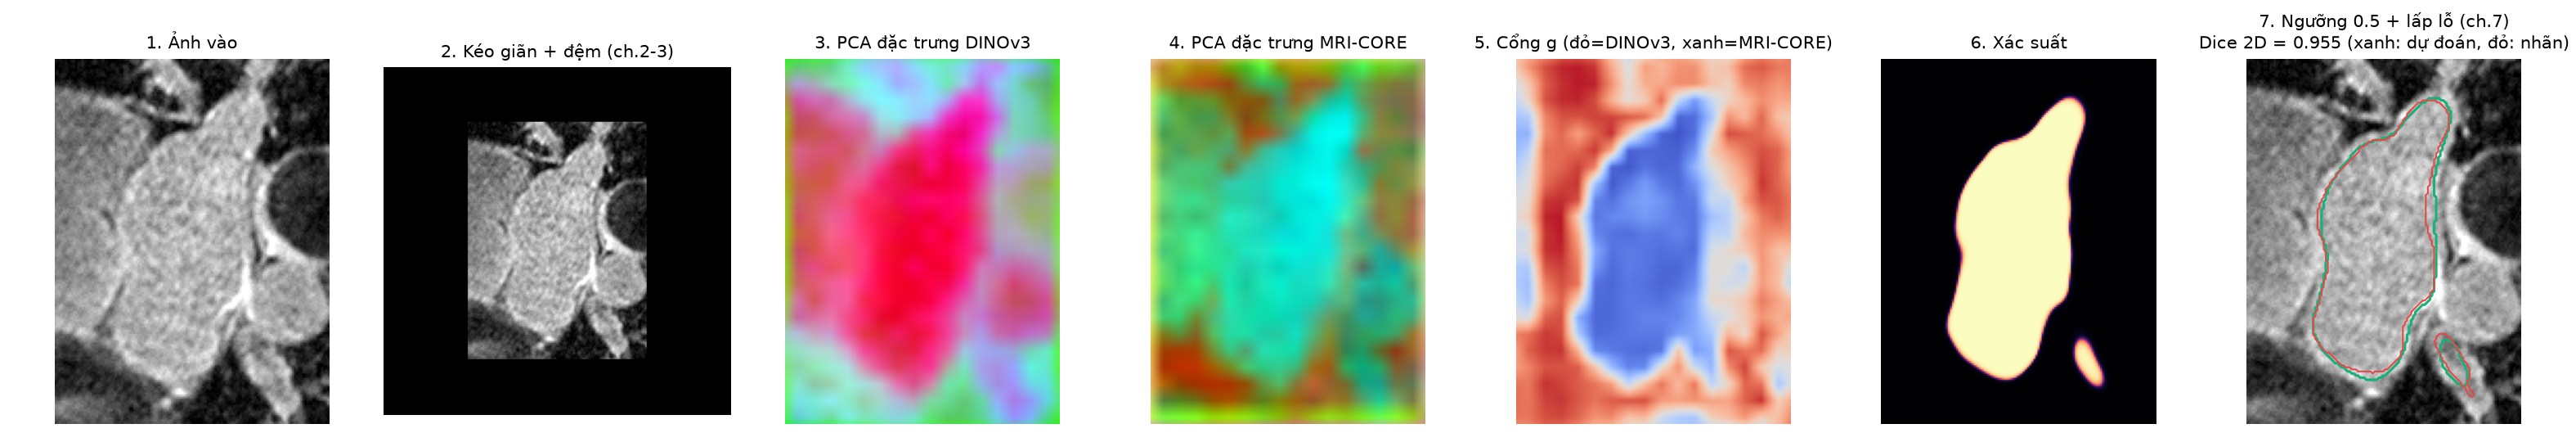
\includegraphics[width=\linewidth]{demo_UPT6DX9I_z52_img.png}\\[1mm]
\begin{itemize}\footnotesize
\item Ảnh \textbf{không bị co}: đệm vào khung 256, phóng $\times2$ $\Rightarrow$ lưới token $32\times32$ cho cả hai encoder; đặc trưng 8\,800 lát tính \textbf{một lần} ($\sim$10 phút/encoder, Apple M2 Pro)
\item Chỉ học phép chiếu + cổng + decoder: \ParamsGate\,M tham số (U-Net đối chứng: \ParamsUnet\,M)
\end{itemize}
\end{frame}

%---------------------------------------------------------------- 6
\begin{frame}{Mỗi encoder ``nhìn thấy'' gì?}
\begin{columns}[T]
\column{0.5\textwidth}
\centering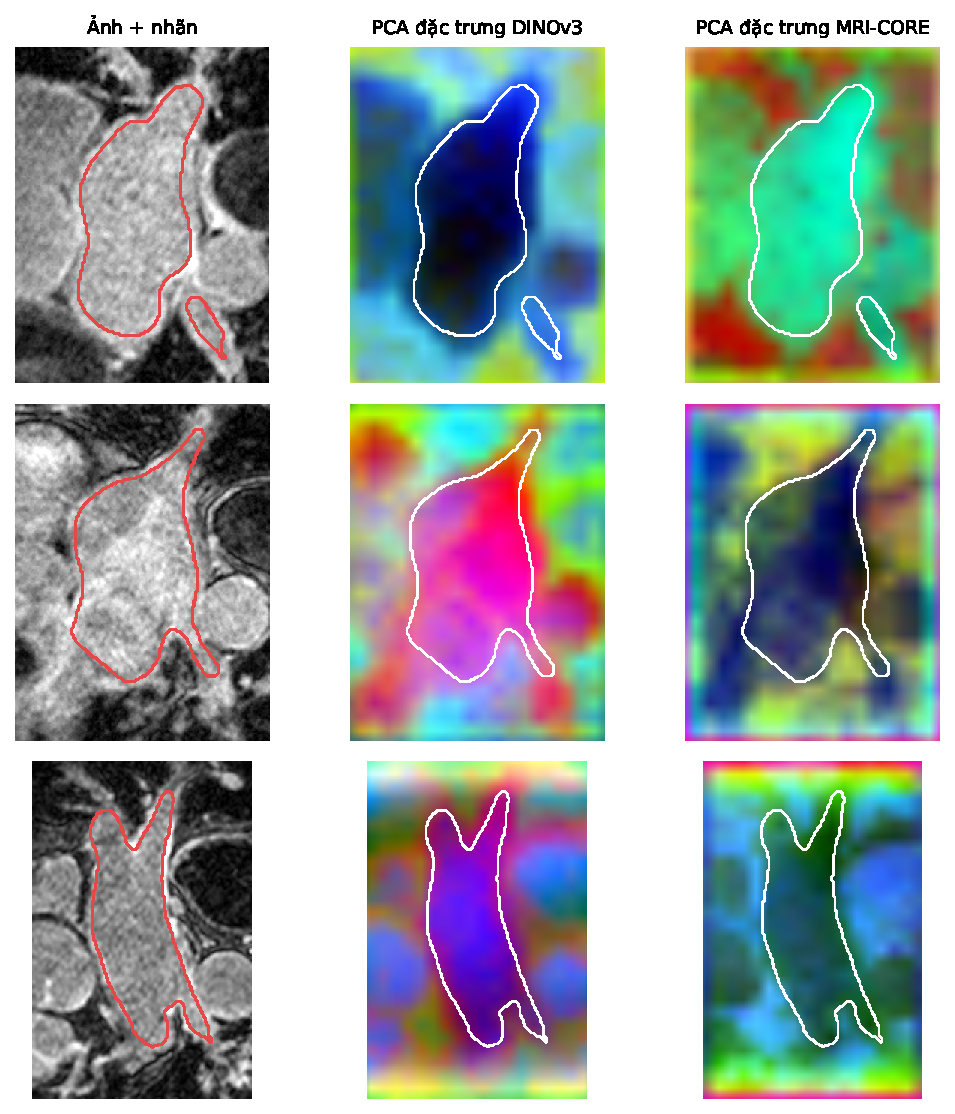
\includegraphics[height=0.82\textheight]{feature_pca.pdf}
\column{0.48\textwidth}
\begin{itemize}
\item PCA 3 thành phần đầu của token (chương 8), sau khi trừ trung bình theo vị trí ô
\item Cả hai đều tách \textbf{tâm nhĩ} thành một vùng đồng nhất mà \emph{không hề} được huấn luyện cho LA
\item DINOv3: ranh giới khối rõ, tách buồng tim lân cận
\item MRI-CORE: nhạy kết cấu/nhiễu MRI hơn
\item[$\Rightarrow$] Hai biểu diễn khác nhau $\Rightarrow$ có cơ sở để ghép
\end{itemize}
\end{columns}
\end{frame}

%---------------------------------------------------------------- 7
\begin{frame}{Thiết lập thực nghiệm và đối chứng}
\begin{columns}[T]
\column{0.5\textwidth}
\hl{Cấu hình (chung decoder, chung ngân sách)}
\begin{itemize}
\item A: chỉ DINOv3 \quad B: chỉ MRI-CORE
\item C: ghép nối + conv $1{\times}1$
\item \textbf{D: GateFuse} (cổng theo điểm ảnh)
\item U-Net 2D học từ đầu (không tiền huấn luyện)
\item Cổ điển: Gauss $\to$ Otsu $\to$ mở $\to$ TPLT trung tâm $\to$ đóng + lấp lỗ
\end{itemize}
\column{0.5\textwidth}
\hl{Huấn luyện \& đánh giá}
\begin{itemize}
\item AdamW, lr $10^{-3}$, cosin; batch 16; 4\,000 vòng (72 khối) / 2\,000 vòng (8 khối)
\item Chọn checkpoint theo Dice 3D validation
\item \textbf{3 seed} mỗi cấu hình, báo cáo TB $\pm$ ĐLC
\item Dice, Jaccard, HD95, ASD trên khối 3D gốc
\item Wilcoxon có dấu trên Dice từng ca
\item Tham số cổ điển dò trên 24 khối train/val (286 bộ)
\end{itemize}
\end{columns}
\end{frame}

%---------------------------------------------------------------- 8
\begin{frame}{Kết quả chính (72 khối huấn luyện, 20 khối test)}
\centering\scriptsize
\resizebox{\linewidth}{!}{\begin{tabular}{lrccccc}
\toprule
Phương pháp & Tham số học & Dice $\uparrow$ & Jaccard $\uparrow$ & HD95 (vx) $\downarrow$ & ASD (vx) $\downarrow$ & $|\Delta V|$ (\%) $\downarrow$\\
\midrule
Cổ điển (Otsu + hình thái) & 0 & 0{,}561 & 0{,}420 & 40{,}69 & 9{,}31 & 54{,}4\\
U-Net 2D (từ đầu) & 1{,}94\,M & 0{,}912{\scriptsize$\pm$0{,}001} & 0{,}838{\scriptsize$\pm$0{,}002} & 8{,}22{\scriptsize$\pm$1{,}01} & 1{,}71{\scriptsize$\pm$0{,}07} & 6{,}5{\scriptsize$\pm$0{,}3}\\
A: DINOv3 & 0{,}20\,M & 0{,}902{\scriptsize$\pm$0{,}002} & 0{,}822{\scriptsize$\pm$0{,}004} & 11{,}02{\scriptsize$\pm$0{,}97} & 1{,}90{\scriptsize$\pm$0{,}10} & \textbf{5{,}9{\scriptsize$\pm$0{,}2}}\\
B: MRI-CORE & 0{,}20\,M & 0{,}908{\scriptsize$\pm$0{,}001} & 0{,}832{\scriptsize$\pm$0{,}001} & 7{,}82{\scriptsize$\pm$0{,}16} & 1{,}66{\scriptsize$\pm$0{,}02} & 7{,}2{\scriptsize$\pm$0{,}5}\\
C: Ghép nối & 0{,}33\,M & 0{,}912{\scriptsize$\pm$0{,}001} & 0{,}839{\scriptsize$\pm$0{,}002} & 8{,}13{\scriptsize$\pm$0{,}56} & 1{,}64{\scriptsize$\pm$0{,}06} & 6{,}1{\scriptsize$\pm$0{,}9}\\
\textbf{D: GateFuse (đề xuất)} & 0{,}30\,M & 0{,}911{\scriptsize$\pm$0{,}002} & 0{,}838{\scriptsize$\pm$0{,}004} & \textbf{7{,}43{\scriptsize$\pm$1{,}03}} & 1{,}60{\scriptsize$\pm$0{,}10} & 6{,}2{\scriptsize$\pm$0{,}4}\\
\textbf{D+: GateFuse + nhánh Sobel} & 0{,}30\,M & \textbf{0{,}913{\scriptsize$\pm$0{,}001}} & \textbf{0{,}840{\scriptsize$\pm$0{,}001}} & 7{,}52{\scriptsize$\pm$0{,}48} & \textbf{1{,}57{\scriptsize$\pm$0{,}03}} & 6{,}6{\scriptsize$\pm$0{,}8}\\
\bottomrule
\end{tabular}}
\vspace{2mm}
\begin{itemize}\small
\item Cổ điển chỉ \DiceClassicalFull: máu trong nhĩ \emph{không tách được} khỏi cấu trúc lân cận bằng cường độ
\item \hl{RQ1}: MRI-CORE $>$ DINOv3 (\DiceMriFull{} vs \DiceDinoFull, $p\PMriVsDinoFull$); biên tốt hơn rõ (HD95 \HdMriFull{} vs \HdDinoFull)
\item \hl{RQ2}: GateFuse $>$ từng encoder (thắng MRI-CORE \WinGateVsMriFull{} ca, $p\PGateVsMriFull$); ngang ghép nối về Dice
\item Đủ nhãn: U-Net học từ đầu bắt kịp (\DiceUnetFull); D+ cao nhất \DiceGateEdgeFull{} nhưng khác biệt chưa có ý nghĩa thống kê
\end{itemize}
\end{frame}

%---------------------------------------------------------------- 9
\begin{frame}{Kết quả định tính}
\centering
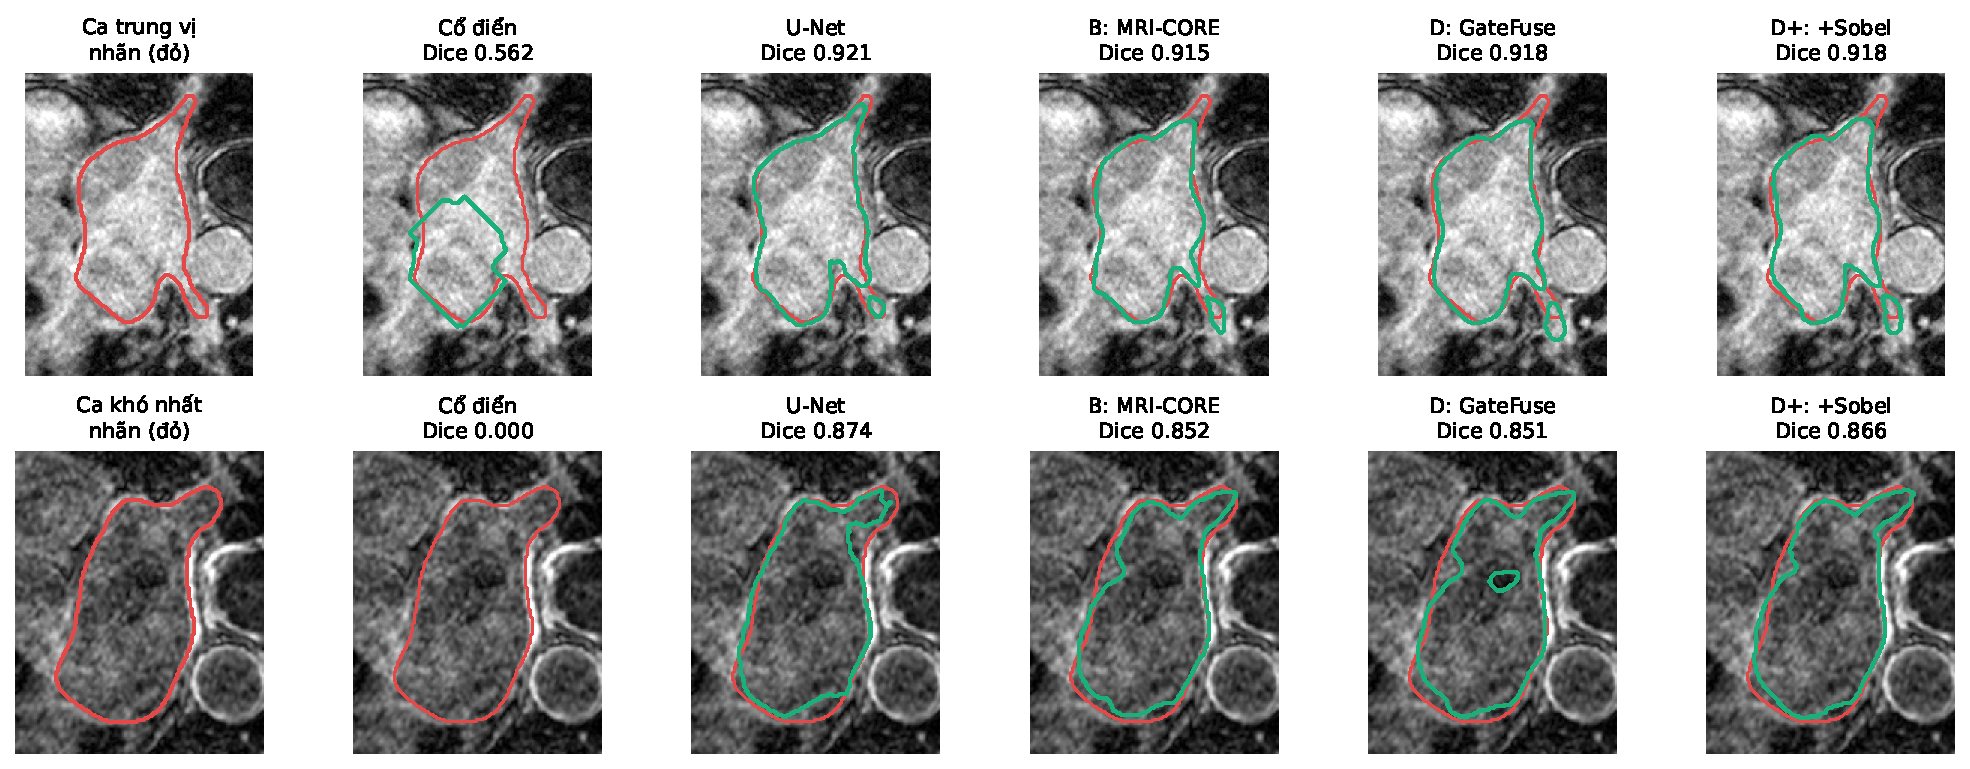
\includegraphics[width=\linewidth,height=0.78\textheight,keepaspectratio]{qualitative_slide.pdf}\\
{\scriptsize\color{ink2} Đỏ: nhãn chuyên gia, xanh: dự đoán (seed 0). Lát có diện tích tâm nhĩ lớn nhất của mỗi ca.}
\end{frame}

%---------------------------------------------------------------- 10
\begin{frame}{Cổng tin encoder nào, ở đâu? (RQ3)}
\begin{columns}[T]
\column{0.58\textwidth}
\centering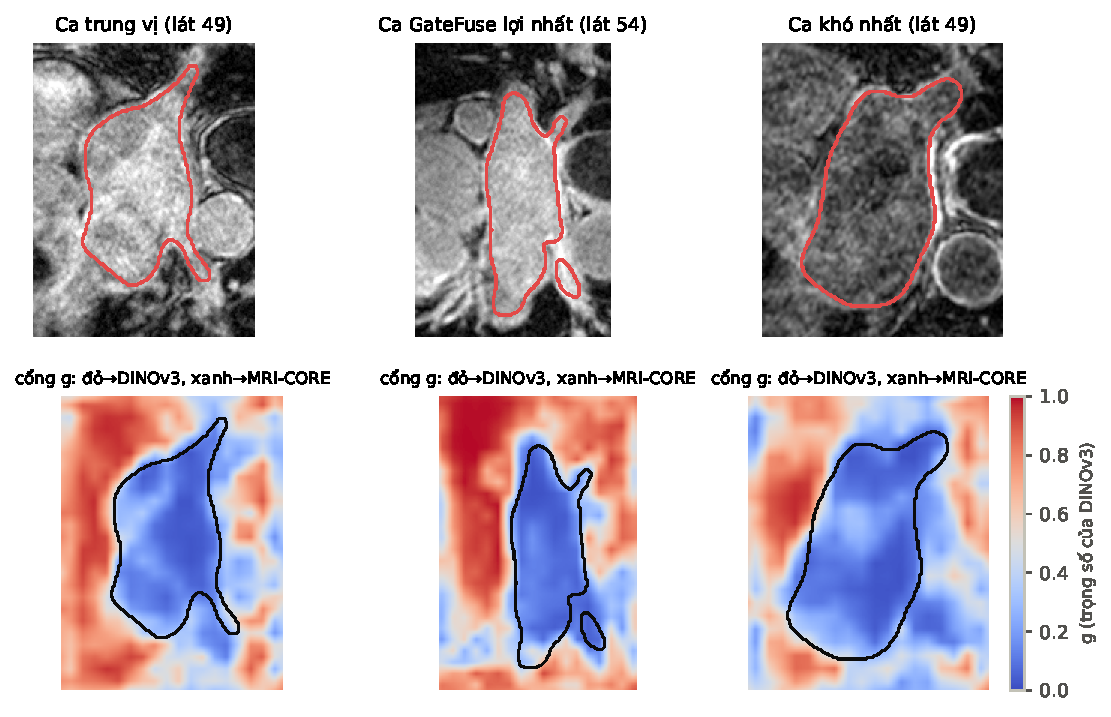
\includegraphics[width=\linewidth]{gate_maps.pdf}
\column{0.4\textwidth}
\centering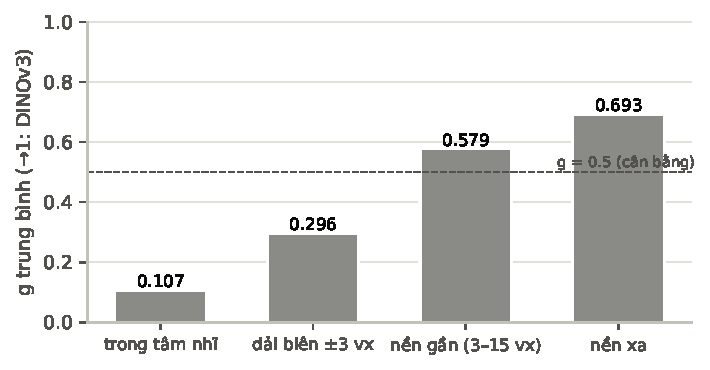
\includegraphics[width=\linewidth]{gate_regions.pdf}
\begin{itemize}\small
\item Trong tâm nhĩ: $g=\GateInside$ $\Rightarrow$ gần như chỉ dùng \textbf{MRI-CORE}
\item Dải biên: $g=\GateBoundary$
\item Nền gần / xa: $g=\GateNear$ / \GateFar{} $\Rightarrow$ nghiêng về \textbf{DINOv3}
\item[$\Rightarrow$] MRI-CORE trả lời ``có phải máu trong nhĩ?'', DINOv3 cho ngữ cảnh hình dạng
\end{itemize}
\end{columns}
\end{frame}

%---------------------------------------------------------------- 11
\begin{frame}{Khi chỉ có 8 khối có nhãn (RQ4)}
\begin{columns}[T]
\column{0.55\textwidth}
\centering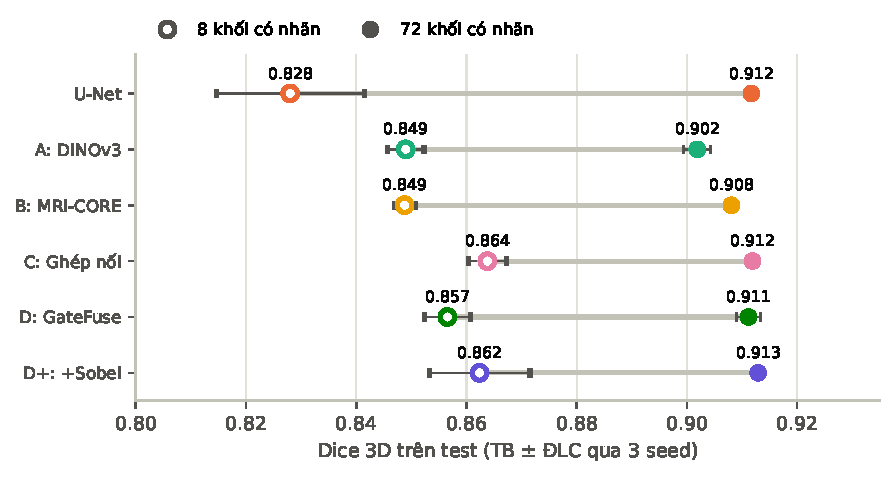
\includegraphics[width=\linewidth]{label_efficiency.pdf}
\column{0.43\textwidth}
\begin{itemize}\small
\item U-Net tụt mạnh nhất: \DiceUnetFull{} $\to$ \DiceUnetFew{} và dao động giữa các seed ($\pm$\DiceSdUnetFew)
\item Đặc trưng nền tảng giữ được 0,85--0,86
\item D+ hơn U-Net \DiffGateEdgeVsUnetFew{} Dice ($p\PGateEdgeVsUnetFew$), GateFuse hơn \DiffGateVsUnetFew{} ($p\PGateVsUnetFew$)
\item HD95: \HdUnetFew{} $\to$ \HdGateEdgeFew{} voxel; sai số thể tích \VolUnetFew\% $\to$ \VolGateEdgeFew\%
\item Tham khảo: V-Net 3D 8 nhãn $\approx$79--80\%; UA-MT (8 nhãn + 72 không nhãn) 84,25\%
\end{itemize}
\end{columns}
\end{frame}

%---------------------------------------------------------------- 12
\begin{frame}{Xử lý ảnh cổ điển: phép mở và hậu xử lý (chương 7, RQ5)}
\begin{columns}[T]
\column{0.4\textwidth}
\centering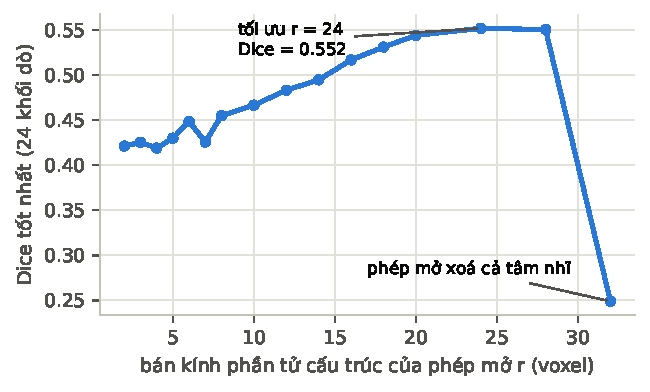
\includegraphics[width=\linewidth]{classical_radius.pdf}\\
{\scriptsize\color{ink2} Pipeline cổ điển: phép mở càng lớn càng cắt được cầu nối với tĩnh mạch phổi, tới khi xoá luôn tâm nhĩ.}
\column{0.58\textwidth}
\centering\footnotesize
\resizebox{\linewidth}{!}{\begin{tabular}{lcccccc}
\toprule
HD95 (voxel) & U-Net & DINOv3 & MRI-CORE & Ghép nối & GateFuse & D+\\
\midrule
Ngưỡng 0{,}5 & 8{,}22 & 11{,}02 & 7{,}82 & 8{,}13 & 7{,}43 & 7{,}52\\
+ TPLT lớn nhất & 6{,}69 & 7{,}90 & 6{,}70 & 7{,}04 & 6{,}24 & 6{,}54\\
+ lấp lỗ & 6{,}65 & 7{,}81 & 6{,}65 & 6{,}95 & 6{,}19 & 6{,}43\\
+ đóng & 6{,}32 & 7{,}10 & 6{,}47 & 6{,}76 & 5{,}82 & 6{,}15\\
\bottomrule
\end{tabular}}
\begin{itemize}\small
\item Giữ TPLT 3D lớn nhất: xoá đốm dương tính giả ở xa
\item + đóng + lấp lỗ: tốt nhất trên \emph{validation} cho mọi mô hình $\Rightarrow$ chọn cho pipeline cuối
\item HD95 giảm 17--36\% (GateFuse: \GatePpRawHd{} $\to$ \GatePpLccFillCloseHd{} voxel)
\item \ErrBand\% voxel sai nằm trong dải $\pm2$ voxel quanh biên (dải chỉ chứa \RefBand\% thể tích nhĩ)
\end{itemize}
\end{columns}
\end{frame}

%---------------------------------------------------------------- 13
\begin{frame}{Thảo luận và hạn chế}
\begin{columns}[T]
\column{0.5\textwidth}
\hl{Trả lời câu hỏi nghiên cứu}
\begin{itemize}\small
\item \textbf{RQ1} Có: đặc trưng MRI tốt hơn, nhất là ở biên
\item \textbf{RQ2} Có: hai đặc trưng bổ sung nhau; cổng $\approx$ ghép nối về Dice nhưng giải thích được
\item \textbf{RQ3} MRI-CORE: bên trong + biên; DINOv3: ngữ cảnh
\item \textbf{RQ4} Lợi thế lớn nhất khi ít nhãn: +3 điểm, ổn định hơn
\item \textbf{RQ5} Hậu xử lý rẻ mà giảm HD95 17--36\%
\item Chi phí: huấn luyện \TrainMsGate{} vs \TrainMsUnet\,ms/vòng; suy luận \InferGate{} vs \InferUnet\,s/khối
\end{itemize}
\column{0.5\textwidth}
\hl{Hạn chế}
\begin{itemize}\small
\item Vùng cắt sẵn lấy từ hộp bao của nhãn (quy ước UA-MT) $\Rightarrow$ bỏ qua bước định vị
\item Mô hình 2D theo lát, encoder đông cứng, không tăng cường dữ liệu
\item Một bộ dữ liệu, một trung tâm; 3 seed
\item Lưới vị trí MRI-CORE được nội suy $14\to32$
\item D+ thiết kế sau khi xem kết quả seed 0 $\Rightarrow$ hậu kiểm
\end{itemize}
\hl{Hướng phát triển}
\begin{itemize}\small
\item Tinh chỉnh LoRA cho encoder; ngữ cảnh 3D
\item Kiểm định ngoài (dữ liệu khác trung tâm)
\end{itemize}
\end{columns}
\end{frame}

%---------------------------------------------------------------- 14
\begin{frame}{Kết luận và demo}
\begin{itemize}
\item Pipeline 5 bước (dữ liệu $\to$ tiền xử lý $\to$ phân đoạn $\to$ hậu xử lý $\to$ đánh giá), đối chứng cổ điển + học sâu, 3 seed, kiểm định thống kê
\item Pipeline cuối (D+ + hậu xử lý): \textbf{Dice \DicePpGateEdgeFull} với 72 khối, \textbf{\DicePpGateEdgeFew} với 8 khối có nhãn
\item Ghép DINOv3 + MRI-CORE tốt hơn từng loại; cổng cho bản đồ giải thích được
\item Ít nhãn: vượt U-Net học từ đầu khoảng 3 điểm Dice
\item Xử lý ảnh cổ điển (kéo giãn, Sobel, mở/đóng, TPLT) hiệu quả nhất khi đặt \emph{quanh} mô hình học
\end{itemize}
\vspace{3mm}
\hl{Chạy thử}\\[1mm]
{\footnotesize\ttfamily python code/demo.py --image samples/<ca>\_img.png --mask samples/<ca>\_mask.png\\
python code/demo.py --h5 samples/volume\_UPT6DX9I.h5}\\[3mm]
{\small\color{ink2} Phân công và khai báo sử dụng AI (Claude, Anthropic): xem mục 9--10 của báo cáo.}
\end{frame}

\end{document}
